\begin{figure}[H]
	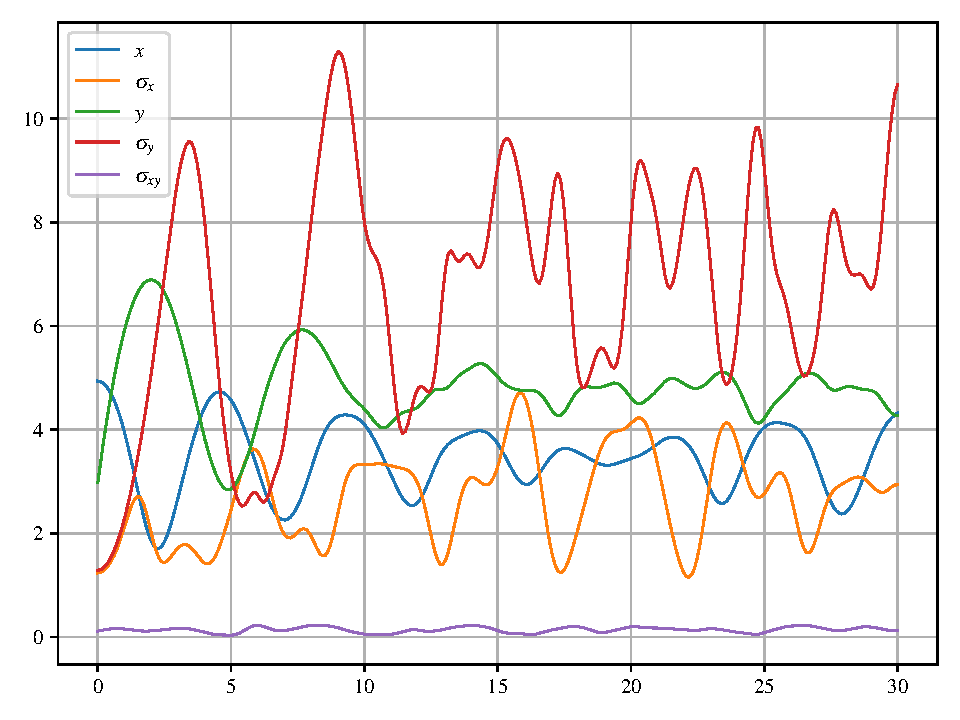
\includegraphics[scale=1]{./figs/expectations.pdf}
	\caption{Várható értékek és szórások időfejlődése}
\end{figure}


\begin{lstlisting}[language=Python]
def convergenceImproved(E):
    G0 = test.G0(x, y, E - test.F * test.L / 2)
    VG0 = (test.F * x - test.F * test.L / 2) * G0 / N * test.L
    realG = test.G(x, y, E)
    G = G0
    norm0 = dx * np.linalg.norm(G0 @ VG0, ord=2)
    norms = np.array([norm0])
    steps = np.array([0])
    for i in range(20):
        Gprev = G
        G = G0 + G @ VG0
        norm = dx * np.linalg.norm(G - realG, ord=2)
        norms = np.append(norms, norm)
        steps = np.append(steps, i+1)
        if norm/norm0 + norm0/norm > 5:
            break
    
    popt, pcov = curve_fit(normguess, steps, norms/norms[0])
    return -popt[0]
\end{lstlisting}